\chapter{Square cylinder}
The square cylinder problem studies the two-dimensional laminar flow around a square cylinder inside a plane channel. The description of the problem can be seen in figure \ref{SchemeSquareProblem}.
\begin{figure}[h]
	\centering
	\includegraphics[scale=0.5]{Square/Definition}
	\caption[General scheme of the square cylinder problem]{General scheme of the square cylinder problem. Extracted from \cite{Breuer2000}}
	\label{SchemeSquareProblem}
\end{figure}

\section{Discretization}
In this kind of problem, the region near the cylinder has an important pressure and velocity gradient whereas in the rest of the channel flow they are smoother. So, near the cylinder a finer mesh is needed, but not in the whole domain of the problem. Using a very fine mesh in all the channel would be computationally expensive and inefficient, but a coarser mesh would lead to inaccurate results, especially in the cylinder.

The domain is divided in three parts, vertically and horizontally. The mesh that contains the obstacle is a uniform mesh of very high precision, whereas the other meshes are also uniform but coarser. The details of the discretization are in table \ref{NumericalCylinder}.
\begin{table}[h]
	\centering
	\begin{tabular}{ |c|c|c|c|c|c|c|c|c|c|c|c|c| }
		\hline
		$N_{1}$ & $N_{2}$ & $N_{3}$ & $M_{1}$ & $M_{2}$ & $M_{3}$ & $D$ & $H$ & $L$ & $l$ & $\rho$ & $u_{max}$ & $\delta$ \\ \hline
		$90$ & $10$ & $300$ & $30$ & $10$ & $30$ & $1$ & $8D$ & $50D$ & $L/4$ & $1$ & $1$ & $10^{-4}$ \\ \hline
	\end{tabular}
\caption{Numerical parameters of the square cylinder problem}
\label{NumericalCylinder}
\end{table}


\section{Boundary conditions}
\subsection{Inlet conditions}
Since the flow is inside a channel, the inflow has a parabolic velocity profile with a maximum velocity $u_{max}$ in the centre:
\begin{equation}
u\left(y\right)=4u_{max}\left[\left(\frac{y}{H}\right)-\left(\frac{y}{H}\right)^{2}\right]
\end{equation}
This maximum velocity defines the Reynolds number of the problem:
\begin{equation}
Re=Re_{max}=\frac{\rho u_{max}D}{\mu}
\end{equation}
As for the pressure conditions, a Neumann condition is imposed:
\begin{equation}
\frac{\partial p}{\partial x}=0
\end{equation}

\subsection{Outlet conditions}
In order to have a developed flow in the outlet, it is important to have a distance large enough between the position of the cylinder and the end of the channel in order to have fully developed flow. To define the outflow, a convective boundary condition is used:
\begin{equation}
\frac{\partial u}{\partial t}+u_{conv}\frac{\partial u}{\partial x}=0
\end{equation}
where $u_{conv}$ is equal to the maximum velocity $u_{max}$ of the parabolic inflow velocity profile. The integration over time of this condition is done using an Adams-Bashforth scheme.

In the outlet, as opposite to the inlet, a Dirichlet condition is used to determine the pressure:
\begin{equation}
p=0
\end{equation}

\subsection{Wall conditions}
In the channel walls the no-slip condition is applied:
\begin{equation}
\vec{v}=0
\label{noslip}
\end{equation}
As well as the boundary layer condition, in which the pressure gradient normal to the wall is 0.

In the convection problems studied in the previous sections the flow was developing inside a cavity with no other obstacles than the walls. In this problem, the fluid flows around a square cylinder, so the boundary conditions have to be also implemented for the cylinder. Since it is a solid object and it does not allow air to flow through it, it is treated as a wall \cite{Ferziger2002}. Consequently the velocity in its boundary is also given by equation \ref{noslip}.

\section{Algorithm}
The algorithm used in the resolution of this problem is the same used in the calculation of the driven cavity problem (section \ref{AlgorithmDriven}).

\section{Results}
Depending on the Reynolds number the wake of the cylinder is completely different. In order to present the results, the fluid is only studied for $1\leq Re<60$, the steady regime. For $Re\geq60$ the fluid does not reach a steady state and the results would not be accurate.

\begin{figure}[h]
	\centering
	\begin{subfigure}{0.5\textwidth}
		\resizebox{1.1\textwidth}{!}{\input{Square/u1}}
		\caption{$Re=1$}
	\end{subfigure}%
	\begin{subfigure}{0.5\textwidth}
		\resizebox{1.1\textwidth}{!}{\input{Square/u3}}
		\caption{$Re=3$}
	\end{subfigure}
	\begin{subfigure}{0.5\textwidth}
		\resizebox{1.1\textwidth}{!}{\input{Square/u5}}
		\caption{$Re=5$}
	\end{subfigure}%
	\begin{subfigure}{0.5\textwidth}
		\resizebox{1.1\textwidth}{!}{\input{Square/u10}}
		\caption{$Re=10$}
	\end{subfigure}
	\begin{subfigure}{0.5\textwidth}
		\resizebox{1.1\textwidth}{!}{\input{Square/u30}}
		\caption{$Re=30$}
	\end{subfigure}%
	\begin{subfigure}{0.5\textwidth}
		\resizebox{1.1\textwidth}{!}{\input{Square/u50}}
		\caption{$Re=50$}
	\end{subfigure}
\caption{Horizontal velocity near the cylinder}
\label{HorizontalCylinder}
\end{figure}

\begin{figure}[h]
	\centering
	\begin{subfigure}{0.5\textwidth}
		\resizebox{1.1\textwidth}{!}{\input{Square/v1}}
		\caption{$Re=1$}
	\end{subfigure}%
	\begin{subfigure}{0.5\textwidth}
		\resizebox{1.1\textwidth}{!}{\input{Square/v3}}
		\caption{$Re=3$}
	\end{subfigure}
	\begin{subfigure}{0.5\textwidth}
		\resizebox{1.1\textwidth}{!}{\input{Square/v5}}
		\caption{$Re=5$}
	\end{subfigure}%
	\begin{subfigure}{0.5\textwidth}
		\resizebox{1.1\textwidth}{!}{\input{Square/v10}}
		\caption{$Re=10$}
	\end{subfigure}
	\begin{subfigure}{0.5\textwidth}
		\resizebox{1.1\textwidth}{!}{\input{Square/v30}}
		\caption{$Re=30$}
	\end{subfigure}%
	\begin{subfigure}{0.5\textwidth}
		\resizebox{1.1\textwidth}{!}{\input{Square/v50}}
		\caption{$Re=50$}
	\end{subfigure}
	\caption{Vertical velocity near the cylinder}
	\label{VerticalCylinder}
\end{figure}

\begin{figure}[h]
	\centering
	\begin{subfigure}{0.5\textwidth}
		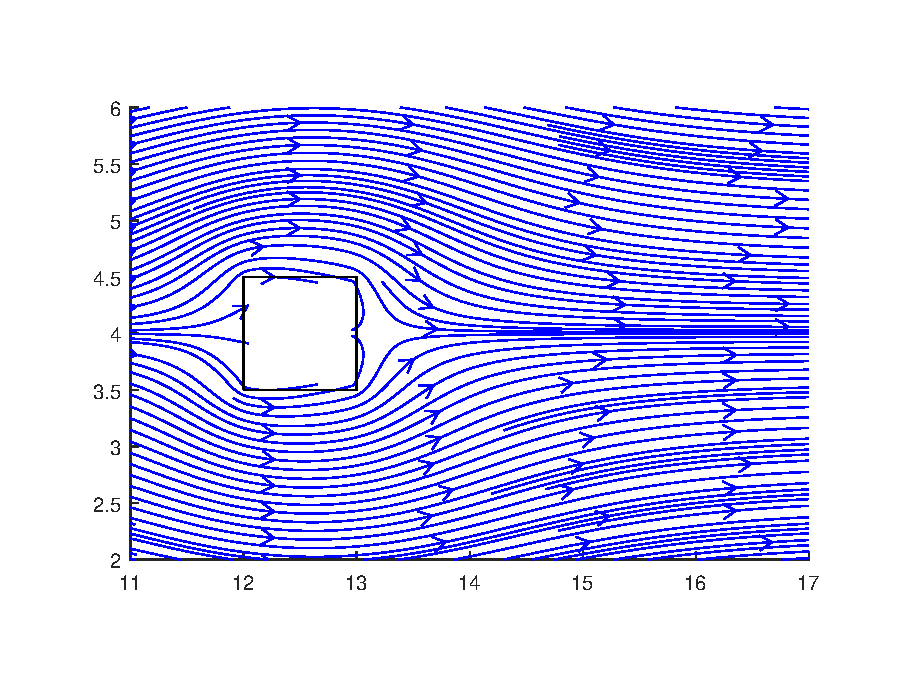
\includegraphics[scale=0.61]{Square/1}
		\caption{$Re=1$}
	\end{subfigure}%
	\begin{subfigure}{0.5\textwidth}
		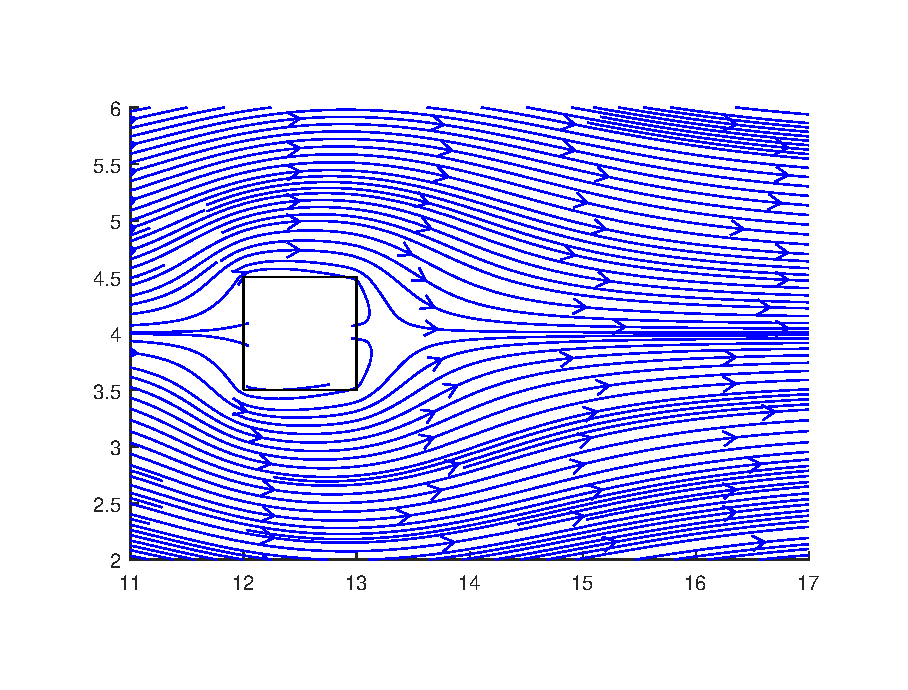
\includegraphics[scale=0.61]{Square/3}
		\caption{$Re=3$}
	\end{subfigure}
	\begin{subfigure}{0.5\textwidth}
		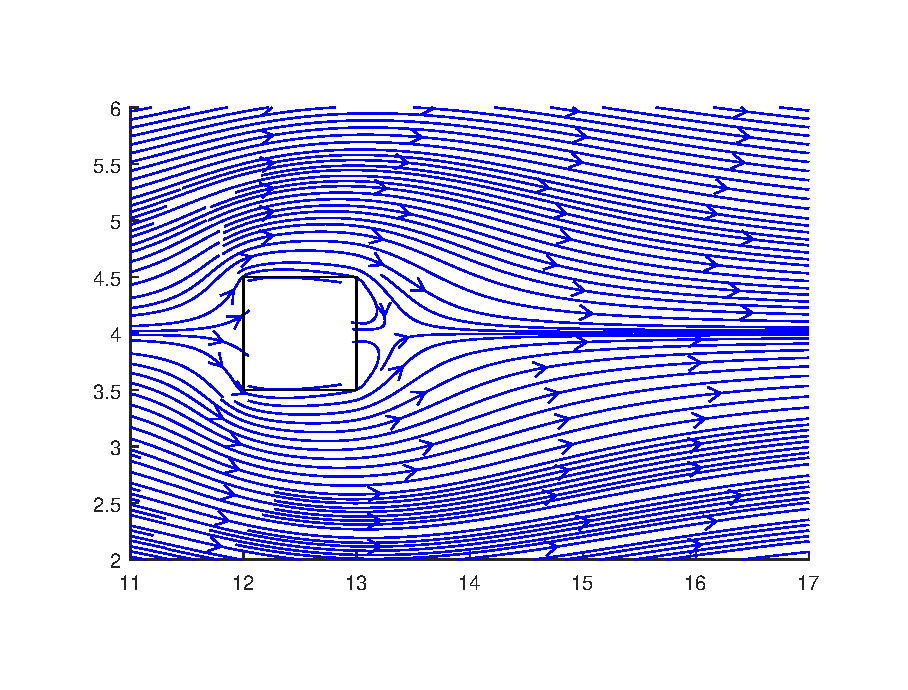
\includegraphics[scale=0.61]{Square/5}
		\caption{$Re=5$}
	\end{subfigure}%
	\begin{subfigure}{0.5\textwidth}
		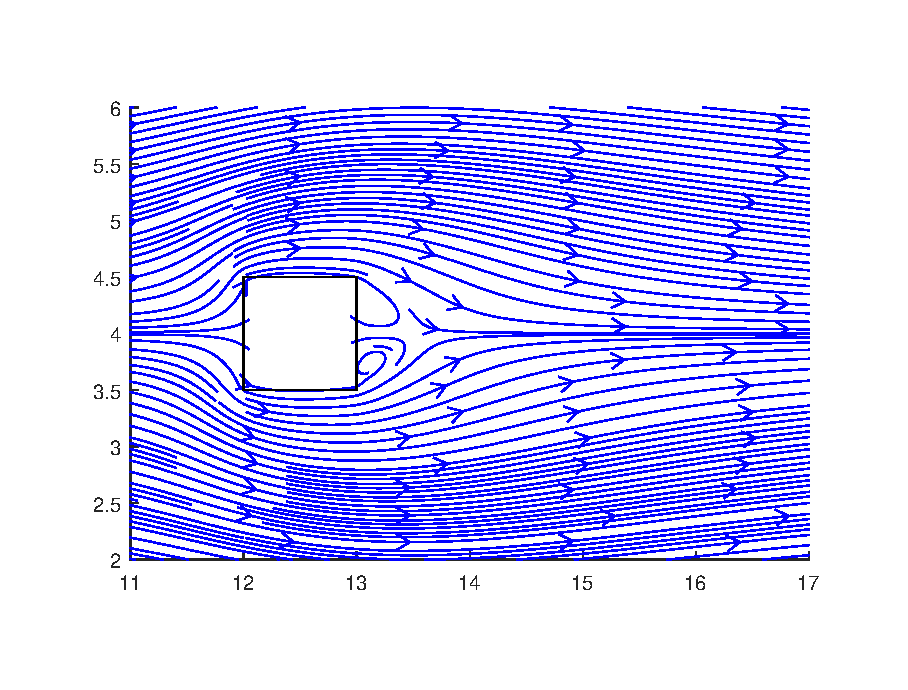
\includegraphics[scale=0.61]{Square/10}
		\caption{$Re=10$}
	\end{subfigure}
	\begin{subfigure}{0.5\textwidth}
		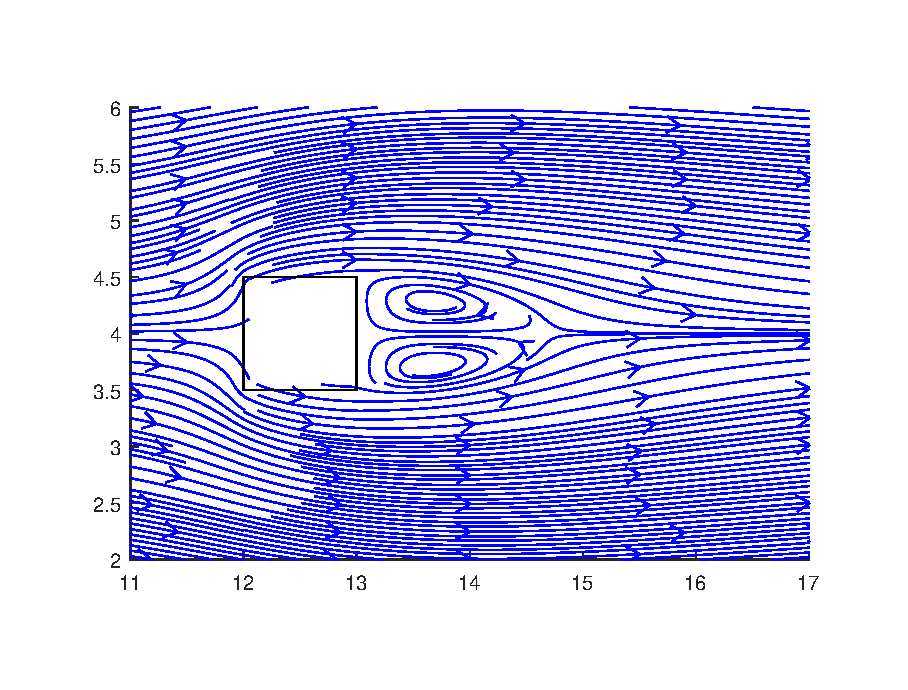
\includegraphics[scale=0.61]{Square/30}
		\caption{$Re=30$}
	\end{subfigure}%
	\begin{subfigure}{0.5\textwidth}
		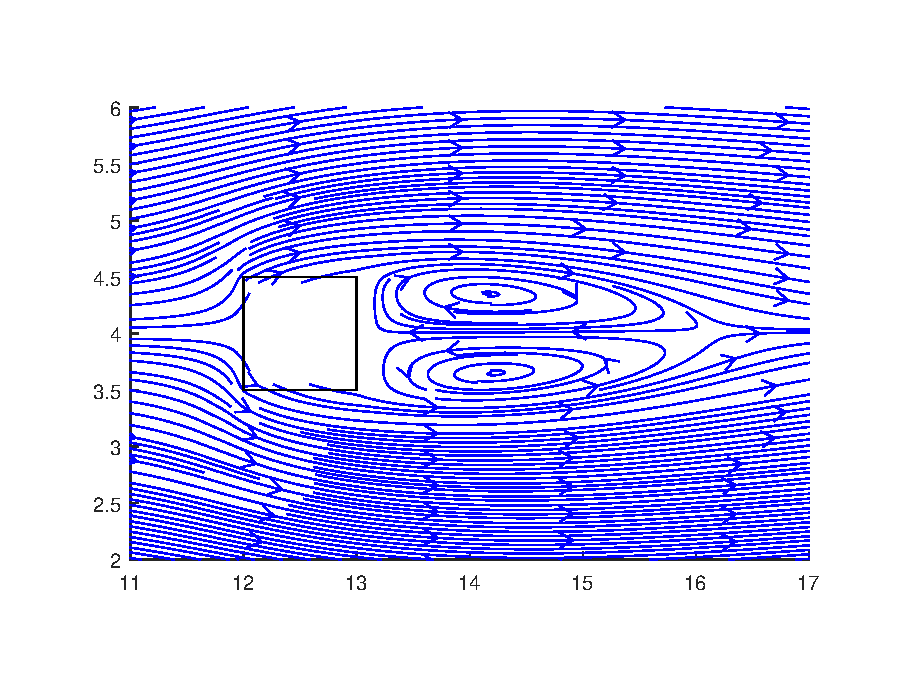
\includegraphics[scale=0.61]{Square/50}
		\caption{$Re=50$}
	\end{subfigure}
	\caption{Vertical velocity near the cylinder}
	\label{StreamlinesCylinder}
\end{figure}